\documentclass[12pt,letterpaper]{article}
\usepackage[utf8]{inputenc}

% Ajustamos los márgenes para corregir las advertencias de fancyhdr
\usepackage[letterpaper, margin=1in, bottom=3in, top=2.2in]{geometry}

% Cargamos primero el paquete fancyhdr
\usepackage{fancyhdr}
% Corregimos los parámetros headheight y footskip
\setlength{\headheight}{15pt} % Al menos 14.49998pt según la advertencia
\setlength{\footskip}{72pt}   % Al menos 71.60547pt según la advertencia

\usepackage{xcolor}
\usepackage{amsmath}
\usepackage{anyfontsize}
\usepackage{graphicx}
\usepackage{tikz} % Necesario para los elementos gráficos
\usepackage{listings} % Para resaltado de sintaxis
\usepackage{sourcesanspro}
\renewcommand{\familydefault}{\sfdefault}
\usepackage{fontawesome5}
\usepackage{titlesec}
\usepackage{setspace}
\usepackage{hyperref}
\usepackage{mdframed} % Para marcos más estables
\usepackage{qrcode} % Paquete para generar códigos QR
\usepackage{eso-pic}
\usepackage{float}

\floatplacement{figure}{H}

% Cargar tikz y la biblioteca de cajitas para mdframed
\usetikzlibrary{calc,shapes,positioning}

% IMPORTANT: Force the text color to be white for the entire document
\AtBeginDocument{\color{primaryColor}}

% Colors updated with better contrast
\definecolor{myblue}{cmyk}{1.0,0.8,0.05,0.20}
\definecolor{bgColor}{RGB}{15, 22, 36}  % Very dark blue, almost black background
\definecolor{primaryColor}{RGB}{255, 255, 255}  % White text - full white for better contrast
\definecolor{accentColor}{RGB}{255, 212, 59}  % Python Yellow
\definecolor{pythonBlue}{RGB}{120, 180, 255}  % Azul Python más claro para mejor contraste
\definecolor{secondaryColor}{RGB}{220, 230, 240}  % Lighter blue-gray for better contrast
\definecolor{terminalBg}{RGB}{22, 22, 22}  % Terminal background remains dark
\definecolor{terminalFrame}{RGB}{40, 40, 40}  % Terminal frame slightly darker
\definecolor{lineNumberColor}{RGB}{100, 100, 100}  % Color más sutil para los números de línea
\definecolor{dividerColor}{RGB}{60, 70, 90}  % Color más sutil para la línea divisoria

% Colores mejorados para el código con mayor contraste
\definecolor{codeTextColor}{RGB}{255, 255, 255}  % Blanco puro para el texto básico
\definecolor{codeKeywordColor}{RGB}{135, 206, 250}  % Azul cielo para palabras clave
\definecolor{codeCommentColor}{RGB}{144, 238, 144}  % Verde claro para comentarios
\definecolor{codeStringColor}{RGB}{255, 215, 135}  % Amarillo para strings
\definecolor{codeMethodColor}{RGB}{255, 160, 122}  % Naranja claro para métodos
\definecolor{codeFunctionColor}{RGB}{255, 215, 0}  % Dorado para funciones
\definecolor{codeNumberColor}{RGB}{255, 255, 150}  % Amarillo claro para números

% Set page background color
\pagecolor{bgColor}

% Hyperref configuration
\hypersetup{
    colorlinks=true,
    linkcolor=accentColor,
    filecolor=accentColor,
    urlcolor=accentColor,
}

% Configuración básica para listings que evita problemas con saltos de página
\lstset{
  language=Python,
  basicstyle=\normalsize\ttfamily\bfseries\color{codeTextColor}, % Tamaño reducido, en blanco y negrita
  backgroundcolor=\color{terminalBg},
  commentstyle=\color{codeCommentColor},
  keywordstyle=\color{codeKeywordColor},
  stringstyle=\color{codeStringColor},
  numberstyle=\color{lineNumberColor}, % Números de línea más sutiles
  breaklines=true,
  breakatwhitespace=true,
  tabsize=4,
  showstringspaces=false,
  frame=none,
  xleftmargin=15pt,
  xrightmargin=0pt,
  aboveskip=10pt,
  belowskip=10pt,
  numbers=left,
  numbersep=8pt,
  extendedchars=true,
  keepspaces=true,
  columns=flexible,
  lineskip=6pt, % Espacio entre líneas ligeramente reducido
  % Keywords de Python (palabras reservadas)
  morekeywords={self, yield, lambda, with, as, from, True, False, None, import, in, for, 
                if, elif, else, while, return, def, class, try, except, finally, raise, 
                break, continue, global, nonlocal, pass, assert, del, yield from},
  % Funciones incorporadas resaltadas de manera distinta
  emph={[2]print,range,sum,int,str,float,list,dict,set,tuple,next,len,type,map,filter,
         reduce,zip,enumerate,sorted,reversed,min,max,open,any,all},
  emphstyle={[2]\color{codeFunctionColor}}
}

% TERMINAL ESTILO MAC MEJORADA CON BOTONES A LA IZQUIERDA Y MENOS ESPACIO SUPERIOR
\newenvironment{macterminal}{%
    \begin{mdframed}[
        linecolor=terminalFrame,
        backgroundcolor=terminalBg,
        roundcorner=5pt,
        skipabove=10pt,
        skipbelow=10pt,
        linewidth=1pt,
        innertopmargin=10pt, % Reducido
        frametitle={%
            \tikz[baseline=(current bounding box.east), outer sep=0pt]{
                \fill[red!80!black] (0,0) circle (5pt);
                \fill[yellow!80!black] (0.7,0) circle (5pt);
                \fill[green!70!black] (1.4,0) circle (5pt);
            }
        },
        frametitlealignment=\raggedright, % Alineado a la izquierda
        frametitleaboveskip=8pt, % Espacio entre el título y el borde superior
        frametitlebelowskip=0pt, % Reducir el espacio entre el título y el contenido
    ]
    % No necesitamos más espacio vertical aquí
}{%
    \end{mdframed}%
}

% Utilities
\newcommand{\verspace}{\vspace{10pt}}

% Section styling - Esquema más elegante y mejorado contraste
\titleformat{\section}
  {\LARGE\bfseries\color{primaryColor}} % Secciones principales en blanco para mejor contraste y más grandes
  {\thesection. }
  {0pt}
  {}
  []

\titleformat{\subsection}
  {\Large\bfseries\color{accentColor}} % Subsecciones en amarillo Python y más grandes
  {\thesubsection. }
  {0pt}
  {}
  []

\titleformat{\subsubsection}
  {\large\bfseries\color{pythonBlue}} % Subsubsecciones en azul Python más claro y más grandes
  {\thesubsubsection. }
  {0pt}
  {}
  []

% Spacing for sections
\titlespacing*{\section}{0pt}{20pt}{10pt}
\titlespacing*{\subsection}{0pt}{15pt}{7pt}
\titlespacing*{\subsubsection}{0pt}{10pt}{5pt}

% Configure header and footer
\pagestyle{fancy}
\fancyhf{}

% Crear un encabezado elegante para todas las páginas (excepto la portada)
\fancyhead[L]{
    
\begin{tikzpicture}[remember picture, overlay]
        % Rectángulo de fondo para la sección Python
        \fill[pythonBlue, rounded corners=3pt] (0,0) rectangle (2.2cm,0.7cm);
        % Texto Python
        \node[text=primaryColor, font=\bfseries] at (1.1cm,0.35cm) {PYTHON};
        
        % Pequeño separador
        \fill[secondaryColor] (2.35cm,0.1cm) rectangle (2.40cm,0.6cm);
        
        % Texto Namespaces con el color de acento
        \node[text=accentColor, font=\bfseries, anchor=west] at (2.35cm,0.35cm) {NAMESPACES};
    \end{tikzpicture}
}

% Línea de encabezado
\renewcommand{\headrulewidth}{0pt}

% Configure footer with profile info
\fancyfoot[C]{
    \vspace*{0.2cm}
    \noindent
    \begin{minipage}{\textwidth}
        \begin{flushleft}
            % Profile image placeholder with TikZ
            \raisebox{0.7cm}{
            \begin{tikzpicture}[baseline]
                \path[fill=bgColor] (0,0) circle (0.8cm);
                \clip (0,0) circle (0.8cm);
                \node at (0,0) {
                    % Placeholder for profile image
                    \includegraphics[width=1.6cm,height=1.6cm]{../../Images/profile-image.jpeg}
                };
            \end{tikzpicture}
            }
            \begin{minipage}[b]{0.8\textwidth}
                % Name
                {\large\bfseries\color{primaryColor}Alejandro Sánchez Yalí}
                
                % Professional description
                \par\vspace{1pt}
                {\small\color{secondaryColor}Software Developer | AI \& Blockchain Enthusiast}
                
                % Contact
                \par\vspace{1pt}
                {\small\color{accentColor}\faGlobe\hspace{5pt}\color{secondaryColor}www.asanchezyali.com}
            \end{minipage}
        \end{flushleft}
        \vspace{8pt} % Space at bottom
    \end{minipage}
}

% Estilo para la portada (sin encabezado ni pie de página)
\fancypagestyle{plain}{
    \fancyhf{}
    \renewcommand{\headrulewidth}{0pt}
    \renewcommand{\footrulewidth}{0pt}
}

% Bullet styling for lists
\renewcommand{\labelitemi}{\textcolor{accentColor}{$\bullet$}} % Primer nivel de viñetas en amarillo (mejor contraste)
\renewcommand{\labelitemii}{\textcolor{pythonBlue}{$\circ$}} % Segundo nivel de viñetas en azul

% Aumentar globalmente el tamaño de texto un 20%
\usepackage{relsize}
\AtBeginDocument{\relsize{1}} % Incrementa la fuente en aproximadamente un 20%

% Comando simplificado para la etiqueta Python
\newcommand{\languagetag}[1]{
    \begin{tikzpicture}[baseline]
        \node[fill=pythonBlue, text=primaryColor, rounded corners=5pt, inner sep=7pt] {
            {\normalsize\textbf{#1}}
        };
    \end{tikzpicture}
}

\newcommand{\BackgroundPic}{%
    \put(0,0){%
        \begin{tikzpicture}[remember picture, overlay]
            % Coloca la imagen de fondo que cubra toda la página
            \node[inner sep=0pt] at (current page.center) {
                \includegraphics[width=\paperwidth,height=\paperheight,keepaspectratio=false]{../../Images/Coding in Cyberpunk Style.jpeg}
            };
            
            % Agrega una capa semitransparente oscura sobre la imagen
            \fill[black, opacity=0.7] (current page.south west) rectangle (current page.north east);
        \end{tikzpicture}%
    }%
}


% Alternativa usando una versión modificada de la URL
\newcommand{\elegantqr}[2]{
    \qrcode[height=2.5cm]{#1}
    \\[0.1cm]
    {\hspace{0.2cm}\color{primaryColor}\small #2\par}
}

% Definir el título personalizado con alineación exacta para todos los elementos
\newcommand{\titlepagecontents}{%
    \AddToShipoutPicture*{\BackgroundPic}
    \vspace*{2cm}
    % Asegurar que todos los elementos estén alineados a la izquierda
    \begin{flushleft}
    \languagetag{Python}\\[0.4cm]
    {\fontsize{38}{52}\bfseries\color{primaryColor}Understanding \color{accentColor}Python\\\color{accentColor}Namespaces\par}
    \vspace{0.3cm}
    {\fontsize{18}{52}\color{secondaryColor}How Scope and Variable Resolution Work Under the Hood\par}
    \vspace{0.3cm}
    {\color{secondaryColor}\today\par}
    \vspace{1.8cm}
    % El QR se alineará a la izquierda aunque internamente esté centrado
    \elegantqr{https://github.com/asanchezyali/social-media-posts/tree/main/Python/Namespaces}{Source Code}
    \end{flushleft}
}

% En la página del título, aplicar el contenido sin márgenes adicionales
\makeatletter
\renewcommand{\maketitle}{%
    \begin{titlepage}
    \setlength{\parindent}{0pt}
    \setlength{\leftskip}{0pt}
    \titlepagecontents
    \end{titlepage}
}
\makeatother

\newcommand{\finalpagecontents}{%
    \AddToShipoutPicture*{\BackgroundPic}
    \vspace*{3cm}
    % Left-aligned elements with EXACT same structure as title page
    \begin{flushleft}
    \languagetag{Feedback}\\[0.4cm]
    {\fontsize{46}{52}\bfseries\color{primaryColor}Found this \color{accentColor}helpful?\par}
    \vspace{0.3cm}
    {\fontsize{18}{52}\color{secondaryColor}Save, comment and share\par}  
    \vspace{0.3cm}
    {\color{secondaryColor}\today\par}
    \end{flushleft}
}

\begin{document}
\setlength{\parindent}{0pt}
\begin{titlepage}
    \titlepagecontents
\end{titlepage}

\section{Introduction to Python Namespaces}

In Python, a namespace is a crucial concept that provides the context in which names (such as variables, functions, classes) are stored and retrieved. Namespaces are implemented as dictionaries that map names to objects, allowing Python to organize and access names efficiently. Understanding namespaces is key to writing maintainable Python code, resolving scope issues, and avoiding name collisions.

\subsection{What Are Namespaces?}

A \textbf{\textcolor{accentColor}{namespace}} is a mapping from names to objects. Essentially, it defines which objects can be referred to by which names in a particular context.

\begin{itemize}
    \item Names in Python refer to objects—whether variables, functions, classes, or modules
    \item Different namespaces can use the same name to refer to different objects
    \item Namespaces are created at different times and have different lifetimes
    \item Python uses namespaces to prevent naming conflicts and organize code effectively
\end{itemize}

In real-world terms, namespaces are similar to how we address people by names. Within one family, "Mom" refers to a specific person, while in another family "Mom" refers to a different person. Each family creates its own "namespace" for names like "Mom", "Dad", etc.

\subsection{Types of Namespaces in Python}

Python organizes code using several namespaces, each with different scope and lifetime:

\begin{itemize}
    \item \textbf{\textcolor{pythonBlue}{Built-in Namespace:}} Contains built-in functions and exceptions like \texttt{print()}, \texttt{len()}, and \texttt{TypeError}.
    \item \textbf{\textcolor{pythonBlue}{Global Namespace:}} Created when a module is loaded and lasts until the interpreter terminates.
    \item \textbf{\textcolor{pythonBlue}{Local Namespace:}} Created when a function is called and deleted when the function returns or raises an exception.
    \item \textbf{\textcolor{pythonBlue}{Enclosing Namespace:}} Exists in nested functions, where inner functions have access to names in outer functions.
\end{itemize}

\section{Namespace Examples}

Let's explore namespaces through practical examples.

\subsection{Basic Namespace Example}

The following example demonstrates the fundamental concept of different namespaces in Python:

\begin{macterminal}
\begin{lstlisting}
# The built-in namespace contains functions like print, len, etc.
print("Built-in namespace example:")
print(f"Type of len function: {type(len)}")
print(f"ID of len function: {id(len)}")

# The global namespace of a module
x = 10
y = "hello"

print("\nGlobal namespace example:")
print(f"x = {x}, type: {type(x)}, id: {id(x)}")
print(f"y = {y}, type: {type(y)}, id: {id(y)}")

# Local namespace in a function
def example_function():
    z = 20  # Local variable
    print("\nLocal namespace inside function:")
    print(f"z = {z}, type: {type(z)}, id: {id(z)}")
    
    # We can access global variables from inside a function
    print(f"x from global namespace: {x}")
    
    # But if we create a local variable with the same name,
    # it shadows the global variable
    x = 30  # This creates a new local variable
    print(f"Local x = {x}, type: {type(x)}, id: {id(x)}")

# Call the function
example_function()

# x in the global namespace is not affected
print("\nAfter function call:")
print(f"Global x is still: {x}")
\end{lstlisting}
\end{macterminal}

This example demonstrates three key namespaces:
\begin{itemize}
    \item The \textbf{built-in namespace} containing Python's built-in functions
    \item The \textbf{global namespace} with variables defined at the module level
    \item A \textbf{local namespace} created when the function is called
\end{itemize}

Notice how the local variable \texttt{x} inside the function is completely separate from the global variable \texttt{x}. Each exists in its own namespace, which is why modifying the local \texttt{x} doesn't affect the global \texttt{x}.

\subsection{Name Resolution with LEGB Rule}

Python uses the LEGB rule to determine which object a name refers to:

\begin{macterminal}
\begin{lstlisting}
# Global variable
x = "global x"

def outer_function():
    # Enclosing variable (from inner_function's perspective)
    x = "enclosing x"
    
    def inner_function():
        # Local variable
        x = "local x"
        print(f"Local x in inner_function: {x}")
        
    # Call the inner function
    inner_function()
    print(f"Enclosing x in outer_function: {x}")

# Call the outer function
outer_function()
print(f"Global x: {x}")
\end{lstlisting}
\end{macterminal}

This demonstrates name resolution through:
\begin{itemize}
    \item \textbf{L} - Local: First, Python looks in the local namespace
    \item \textbf{E} - Enclosing: If not found, it searches in the enclosing function's namespace
    \item \textbf{G} - Global: If still not found, it searches the global namespace
    \item \textbf{B} - Built-in: Finally, it looks in the built-in namespace
\end{itemize}

\section{Modifying Variables in Different Namespaces}

Python provides keywords to modify variables in outer namespaces.

\subsection{Using \texttt{global} to Modify Global Variables}

The \texttt{global} keyword allows functions to modify variables in the global namespace:

\begin{macterminal}
\begin{lstlisting}
x = "global x"

# Without global keyword
def function_one():
    x = "local x"  # Creates a new local variable
    print(f"Inside function_one: {x}")

# With global keyword
def function_two():
    global x
    x = "modified global x"  # Modifies the global variable
    print(f"Inside function_two: {x}")

print(f"Before function calls: {x}")
function_one()
print(f"After function_one: {x}")  # Unchanged
function_two()
print(f"After function_two: {x}")  # Changed
\end{lstlisting}
\end{macterminal}

\subsection{Using \texttt{nonlocal} for Enclosing Variables}

The \texttt{nonlocal} keyword allows nested functions to modify variables in enclosing functions:

\begin{macterminal}
\begin{lstlisting}
def outer():
    y = "outer y"
    
    def inner():
        nonlocal y  # This allows us to modify the enclosing variable
        y = "modified by inner()"
        print(f"Inside inner(): {y}")
    
    print(f"Before calling inner(): {y}")
    inner()
    print(f"After calling inner(): {y}")  # Changed

outer()
\end{lstlisting}
\end{macterminal}

\section{Module Namespaces and Imports}

Each Python module has its own global namespace, which is why the same name can be used in different modules without conflict.

\begin{macterminal}
\begin{lstlisting}
# Each module has its own namespace
import math
import random
import datetime as dt

# Different modules can have variables or functions with the same name
# without conflicts, because they exist in separate namespaces

print("Module namespaces:")
print(f"math.pi = {math.pi}")
print(f"sin(30$^\circ$) = {math.sin(math.radians(30))}")

print(f"\nrandom.random() = {random.random()}")
print(f"random choice from list = {random.choice(['apple', 'banana', 'cherry'])}")

# Using an aliased import
current_time = dt.datetime.now()
print(f"\nCurrent time: {current_time}")

# Importing specific items to the local namespace
from math import sqrt, pow
print(f"\nImported directly: sqrt(16) = {sqrt(16)}")
print(f"Imported directly: pow(2, 3) = {pow(2, 3)}")
\end{lstlisting}
\end{macterminal}

Python's import system is closely tied to namespaces:
\begin{itemize}
    \item \texttt{import module}: Keeps names in the module's namespace
    \item \texttt{from module import name}: Brings specific names into the current namespace
    \item \texttt{from module import *}: Brings all names into the current namespace (generally not recommended)
    \item \texttt{import module as alias}: Creates a new name in the current namespace that refers to the module
\end{itemize}

\section{Namespace Collisions and How to Avoid Them}

Name collisions occur when the same name is used to refer to different objects in overlapping namespaces. Let's look at common issues and solutions:

\subsection{Collisions with Built-ins}

One common mistake is reusing names of built-in functions:

\begin{macterminal}
\begin{lstlisting}
# Define a variable with the same name as a built-in function
list = [1, 2, 3, 4, 5]
print(f"Our list variable: {list}")

# Now trying to use the built-in list function will fail
try:
    new_list = list("abcde")  # This will fail
    print(f"New list: {new_list}")
except TypeError as e:
    print(f"Error: {e}")

# Restore the built-in
del list
new_list = list("abcde")  # Now it works
print(f"After restoring built-in: {new_list}")
\end{lstlisting}
\end{macterminal}

\subsection{Import Collisions}

When importing from different modules, name collisions can occur:

\begin{macterminal}
\begin{lstlisting}
# First scenario - same name from different modules
from math import floor
print(f"math.floor(3.7) = {floor(3.7)}")

# If we import a different function with the same name, it overwrites the first one
from statistics import floor
print(f"statistics.floor(3.7) = {floor(3.7)}")  # This is now statistics.floor

# Solution: Use aliases or full module imports
import math
import statistics
print(f"Using full modules - math.floor(3.7) = {math.floor(3.7)}")
print(f"Using full modules - statistics.floor(3.7) = {statistics.floor(3.7)}")
\end{lstlisting}
\end{macterminal}

\section{Class and Instance Namespaces}

Classes introduce their own namespaces, and each instance has its own namespace for instance variables.

\begin{macterminal}
\begin{lstlisting}
class Person:
    species = "Homo sapiens"  # Class variable
    
    def __init__(self, name, age):
        self.name = name  # Instance variable
        self.age = age    # Instance variable
    
    def greet(self):
        # Local variable within the method
        message = f"Hello, my name is {self.name}"
        return message

# Create two instances
alice = Person("Alice", 30)
bob = Person("Bob", 25)

# Class variables are shared
print(f"Person.species: {Person.species}")
print(f"alice.species: {alice.species}")
print(f"bob.species: {bob.species}")

# Instance variables are unique to each instance
print(f"alice.name: {alice.name}")
print(f"bob.name: {bob.name}")
\end{lstlisting}
\end{macterminal}

This demonstrates:
\begin{itemize}
    \item \textbf{Class namespace:} Shared by all instances (e.g., \texttt{species})
    \item \textbf{Instance namespace:} Unique to each instance (e.g., \texttt{name} and \texttt{age})
    \item \textbf{Method namespace:} Local namespace created when a method is called
\end{itemize}

\section{Inspecting Namespaces}

Python provides several tools for inspecting namespaces at runtime.

\begin{macterminal}
\begin{lstlisting}
# Get all variables in the global namespace
global_vars = globals()
print(f"Global namespace has {len(globals())} items")

# Get all local variables in a function
def show_locals():
    x = 10
    y = 20
    local_vars = locals()
    print(f"Local namespace has {len(local_vars)} items")
    print(f"Local variables: {list(local_vars.keys())}")

show_locals()

# Inspect module namespace
import math
print(f"\nMath module has {len(dir(math))} attributes")
print(f"Some math constants: {[name for name in dir(math) if name.isupper()]}")

# Inspect class namespace
class MyClass:
    class_var = "Class variable"
    def method(self):
        pass

print(f"\nMyClass namespace: {[name for name in dir(MyClass) if not name.startswith('__')]}")

# Inspect instance namespace
instance = MyClass()
instance.instance_var = "Instance variable"
print(f"Instance __dict__: {instance.__dict__}")
\end{lstlisting}
\end{macterminal}

These tools are invaluable for debugging namespace issues and understanding code behavior.

\section{Common Namespace Pitfalls}

\subsection{UnboundLocalError}

A common error occurs when trying to modify a global variable without the \texttt{global} keyword:

\begin{macterminal}
\begin{lstlisting}
x = 10

def problematic_function():
    try:
        print(x)  # Try to access global x
        x += 1    # Try to modify it (creates a local variable)
    except UnboundLocalError as e:
        print(f"Error: {e}")
        print("Python sees the assignment and treats x as local,")
        print("but x is not defined before it's used")

problematic_function()

# Solution: Use global keyword
def correct_function():
    global x
    print(f"Global x: {x}")
    x += 1
    print(f"After modification: {x}")

correct_function()
\end{lstlisting}
\end{macterminal}

\subsection{Variable Shadowing}

When local variables have the same name as global or enclosing variables, shadowing occurs:

\begin{macterminal}
\begin{lstlisting}
value = "global"

def outer():
    value = "enclosing"
    
    def inner():
        value = "local"
        print(f"Inner value: {value}")
    
    inner()
    print(f"Outer value: {value}")

outer()
print(f"Global value: {value}")
\end{lstlisting}
\end{macterminal}

This is not necessarily an error, but it can lead to confusion if not well understood.

\section{Best Practices for Working with Namespaces}

To leverage namespaces effectively and avoid common issues:

\begin{itemize}
    \item \textbf{\textcolor{pythonBlue}{Avoid global variables}} when possible. Use function parameters and return values instead.
    \item \textbf{\textcolor{pythonBlue}{Don't override built-in names}} like \texttt{list}, \texttt{dict}, \texttt{sum}, etc.
    \item \textbf{\textcolor{pythonBlue}{Prefer explicit imports}} (\texttt{import module}) over \texttt{from module import *}.
    \item \textbf{\textcolor{pythonBlue}{Use unique, descriptive names}} to reduce the chance of collisions.
    \item \textbf{\textcolor{pythonBlue}{Utilize encapsulation}} with classes to organize related functionality and data.
    \item \textbf{\textcolor{pythonBlue}{Keep the global namespace clean}} by encapsulating code in functions and classes.
    \item \textbf{\textcolor{pythonBlue}{Be cautious}} when using \texttt{global} and \texttt{nonlocal}. They can make code harder to understand.
\end{itemize}

\section{Namespaces in Real-world Applications}

Understanding namespaces is important for several real-world programming scenarios:

\begin{itemize}
    \item \textbf{Creating modules and packages} that can be imported without name conflicts
    \item \textbf{Writing maintainable code} with appropriate variable scoping
    \item \textbf{Debugging issues} related to variable scope and visibility
    \item \textbf{Understanding frameworks} like Django that use namespaces for template variables
    \item \textbf{Managing dependencies} in large applications
    \item \textbf{Creating domain-specific languages} or embedded syntaxes
\end{itemize}

\section{Conclusion}

Python's namespace system is a fundamental feature that provides organization, scope isolation, and name resolution in the language. By understanding how namespaces work, you can write more organized, maintainable, and error-resistant code.

The concept allows Python to separate names in different contexts, preventing conflicts and making large-scale application development possible. Whether you're writing simple scripts or complex frameworks, a solid grasp of namespaces will help you create better Python code.

Remember these key points:
\begin{itemize}
    \item Namespaces provide context for names in Python
    \item The LEGB rule determines how Python resolves names
    \item Different types of namespaces have different lifetimes and accessibility
    \item Python provides tools to inspect and manipulate namespaces at runtime
    \item Understanding namespaces helps avoid common pitfalls like name collisions and scope issues
\end{itemize}

\section{References}

\begin{itemize}
    \item Python Documentation. (2023). \textit{Python Execution Model}. \href{https://docs.python.org/3/reference/executionmodel.html}{Link}
    \item Ramalho, L. (2021). \textit{Fluent Python, 2nd Edition}. O'Reilly Media.
    \item Beazley, D. (2009). \textit{Python Essential Reference, 4th Edition}. Addison-Wesley.
    \item Python PEP 227. (2001). \textit{Statically Nested Scopes}. \href{https://www.python.org/dev/peps/pep-0227/}{Link}
    \item Barry, P. (2016). \textit{Head First Python, 2nd Edition}. O'Reilly Media.
    \item This article was translated, edited and written in collaboration with AI. If you find any inconsistencies or have suggestions for improvement, please don't hesitate to open an issue in our GitHub repository at \href{https://github.com/asanchezyali/social-media-posts}{github} or reach out directly.
\end{itemize}

\section{Explore My Other Posts}
\vspace{10pt}
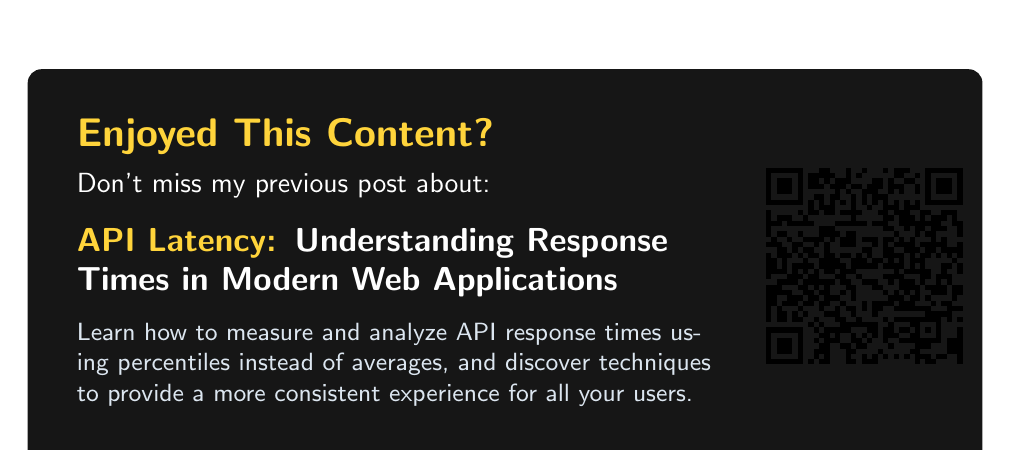
\begin{tikzpicture}
  \fill[color=terminalBg, rounded corners=5pt] (0,0) rectangle (\textwidth,-5);
  \pgfmathsetmacro{\availableWidth}{\textwidth-4cm}
  \begin{scope}
    \node[text=accentColor, font=\Large\bfseries, anchor=north west] at (0.5cm,-0.5cm) {Enjoyed This Content?};
    \node[text=primaryColor, font=\normalsize, anchor=north west] at (0.5cm,-1.2cm) {Don't miss my previous post about:};
    \node[text=secondaryColor, font=\large\bfseries, anchor=north west, text width=\availableWidth] at (0.5cm,-1.9cm) {\color{accentColor}API Latency: \color{primaryColor}Understanding Response Times in Modern Web Applications};
    \node[text=secondaryColor, font=\small, text width=\availableWidth, anchor=north west] at (0.5cm,-3.1cm) {
      Learn how to measure and analyze API response times using percentiles instead of averages,
      and discover techniques to provide a more consistent experience for all your users.
    };
  \end{scope}
  \node[anchor=center] at ({\textwidth-1.5cm}, {-2.5cm}) {
    \qrcode[height=2.5cm]{https://github.com/asanchezyali/social-media-posts/tree/main/Python/FastAPILatency}
  };
\end{tikzpicture}
\vspace{5pt}

\clearpage
\thispagestyle{empty}
\finalpagecontents

\end{document}